\section{Auswertung}
\label{sec:Auswertung}

 Weiterhin muss beachtet werden, dass der Generator einen Innenwiderstand
von $R_i = 600\, \si{\ohm}$ aufweist.
Somit kann also der reale Wert für die Zeitkonstante mit 
\begin{align}

\end{align}




\begin{table}[H]
\normalsize

\centering
\sisetup{table-format=4.0}
\begin{tabular}{c c c c}
\toprule
        Messung & $t \,/\,\si{\milli\second}$ & $U_C \,/\,\si{\volt}$ & $\frac{U_C}{U_0}$ \\
        \midrule

1   & 0      &  9.8   &    1       \\
2   & 0.1    &  8.6   & 0.87755    \\
3   & 0.15   &   8    & 0.81633    \\
4   & 0.5    &   5    & 0.51020    \\
5   & 1      &  2.6   & 0.26531    \\
6   & 1.1    &  2.4   & 0.24489    \\
7   & 1.2    &   2    & 0.20408    \\
8   & 1.5    &  1.3   & 0.13265    \\
9   & 2.3    &  0.4   & 0.04082    \\
10  & 2.95   &  0.2   & 0.02041    \\



     
        

        
\bottomrule
\end{tabular}
\caption{Aufgenommene Werte zur Bestimmung von der Zeitkonstanten des RC-Gliedes}
\label{tab:1}
\end{table}


\begin{figure}
  \centering
  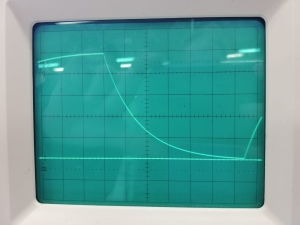
\includegraphics{content/ErsterTeil.jpg}
  \caption{TEXT}
  \label{fig:ErsterTeil}
\end{figure}


Siehe \autoref{fig:plot}!

\begin{table}[H]
\normalsize

\centering
\sisetup{table-format=4.0}
\begin{tabular}{c c c c c c c}
\toprule
        Messung & $U_G \,/\,\si{\volt}$ & $U_C \,/\,\si{\volt}$ & $Frequenz \,/\,\si{\hertz}$ & $a\,/\, \si{\milli\second}$ & $b\,/\, \si{\milli\second}$ & $Phase$ \\
        \midrule
        1   & 5 & 4.9 & 10 & 0.6 & 98 &     0.03847 \\
        2   & 5 & 4.9 & 20 & 1.0 & 50 &     0.12566 \\
        3   & 5 & 4.8 & 30  & 0.8 & 33 &    0.15232 \\ 
        4   & 5 & 4.8 & 40 & 0.76 & 25 &    0.19101 \\
        5   & 5 & 4.8 & 50 & 0.8 & 20 &     0.25132 \\
        6   & 5 & 4.7 & 60 & 0.7 & 16.5 &   0.26656 \\
        7   & 5 & 4.6 & 70 & 0.8 & 14 &     0.35904 \\
        8   & 5 & 4.5 & 80 & 0.8 & 12.4 &   0.40537 \\
        9   & 5 & 4.4 & 90 & 0.8 & 11.2 &   0.44880 \\
        10  & 5 & 4.4 & 100 & 0.7 & 10 &    0.43982 \\
        11  & 5 & 4.2 & 125 & 0.7 & 8 &     0.54978 \\
        12  & 5 & 4.0 & 150 & 0.65 & 6.6 &  0.61880 \\
        13  & 5 & 3.6 & 175 & 0.6 & 5.7 &   0.66139 \\
        14  & 5 & 3.5 & 200 & 0.6 & 5 &     0.75398 \\
        15  & 5 & 2.6 & 300 & 0.5 & 3.3 &   0.95200 \\
        16  & 5 & 2.2 & 400 & 0.4 & 2.5 &   1.00531 \\
        17  & 5 & 1.8 & 500 & 0.4 & 2 &     1.25664 \\
        18  & 5 & 1.2 & 750 & 0.28 & 1.35 & 1.30318 \\
        19  & 5 & 0.95 & 1000 & 0.2 & 1 &   1.25664 \\
        20  & 5 & 0.20 & 5000 & 0.05 & 0.2 & 1.57080 \\
        21  & 5 & 0.10& 10000 & 0.025 & 0.1 & 1.57080 \\



        
\bottomrule

\end{tabular}

\caption{Aufgenommene Werte zur Bestimmung von $R_{11}$}
\label{tab:2}
\end{table}